
\documentclass{beamer}
\usepackage{colortbl}
\usepackage{graphicx}

\usetheme{Antibes}

\title[Statistics and Data Analysis]{A Short Introduction to Statistics and Data Analysis - DRAFT DO NOT CITE OUR QUOTE}
\author{James T. Durant}

\begin{document}

\AtBeginSection[]
{
\begin{frame}
	\frametitle{Outline}
	\tableofcontents[currentsection]
\end{frame}
}


\begin{frame}
\titlepage
\end{frame}

\section{Introduction}
\begin{frame}{Introduction}
Today we will be demonstrating several concepts that we are utilizing in the Exposure Investigation and Data Analysis Team. We will be using \textbf{R} as a platform to demonstrate these concepts. our focus will not be on the mechnics of using \textbf{R} or the underlying mathmatics, but to try and illustrate the concepts of what is happening and basic concepts that will help guide thier use.

 \textbf{R} is not the sole platform that can perform these analyses, but the concepts are transient to all instances.

\alert{Almost all data analysis requires some anaysis and understanding - there are no cookbook techniques }

\end{frame}

\section{Distribution Functions}

\begin{frame}{Emprical Distribution Functions (ECDF)}
\begin{columns}    
	\begin{column}{4cm}        
		\begin{center}
		ECDF Plot           
	 	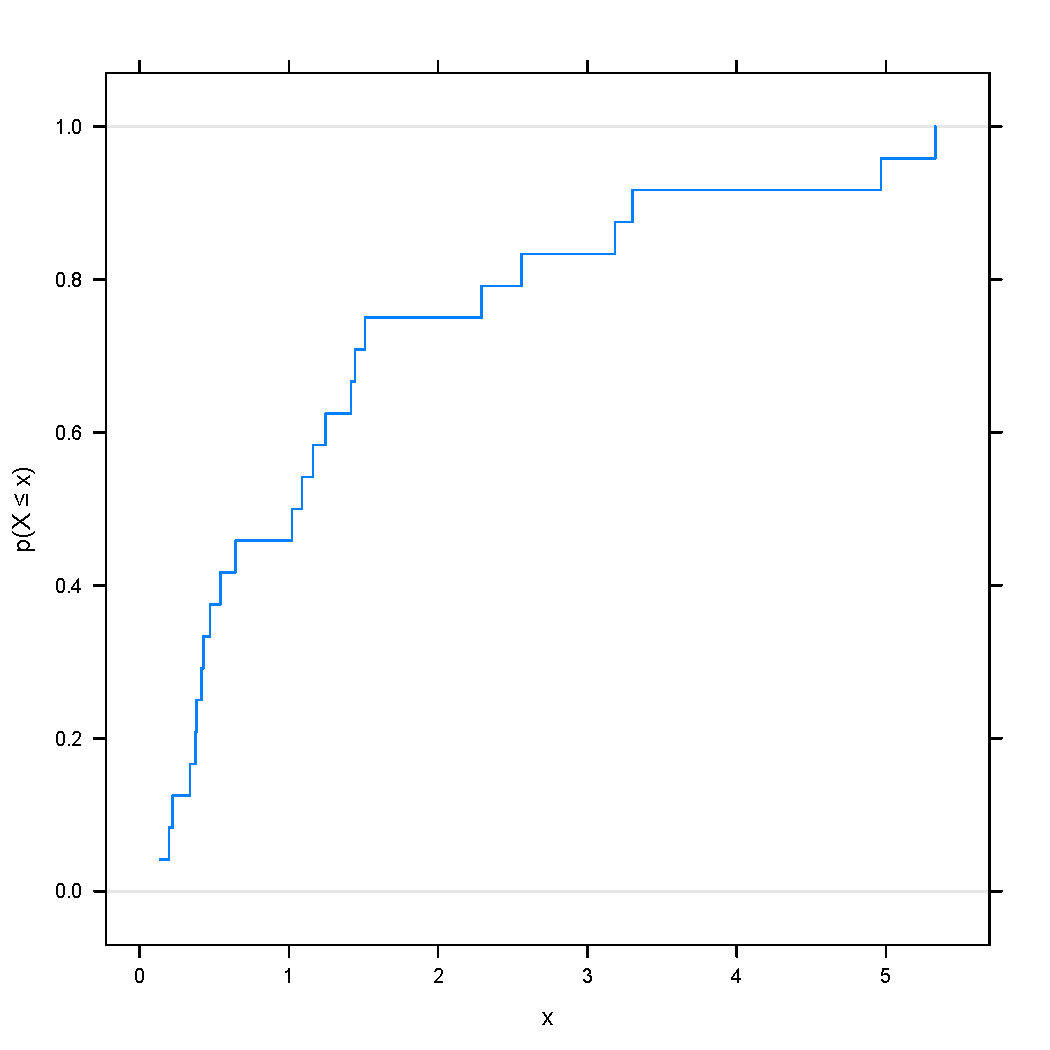
\includegraphics[width=1.0\textwidth]{Figure1}        
		\end{center}   
	 \end{column}    
	\begin{column}{5cm}        
	  
	\begin{itemize}
	\item Probability that a given value is less than a value
	\item Based on actual data - with each point having a probability 1/N where N is sample size.
	\item When plotted looks like stair steps going up from 0 to 1.
	\end{itemize}
	\end{column}
	\end{columns}

\end{frame}

\begin{frame}{Probability Distribution Functions (PDF)}
\begin{columns}    
	\begin{column}{4cm}        
		\begin{center}
		PDF Plot           
	 	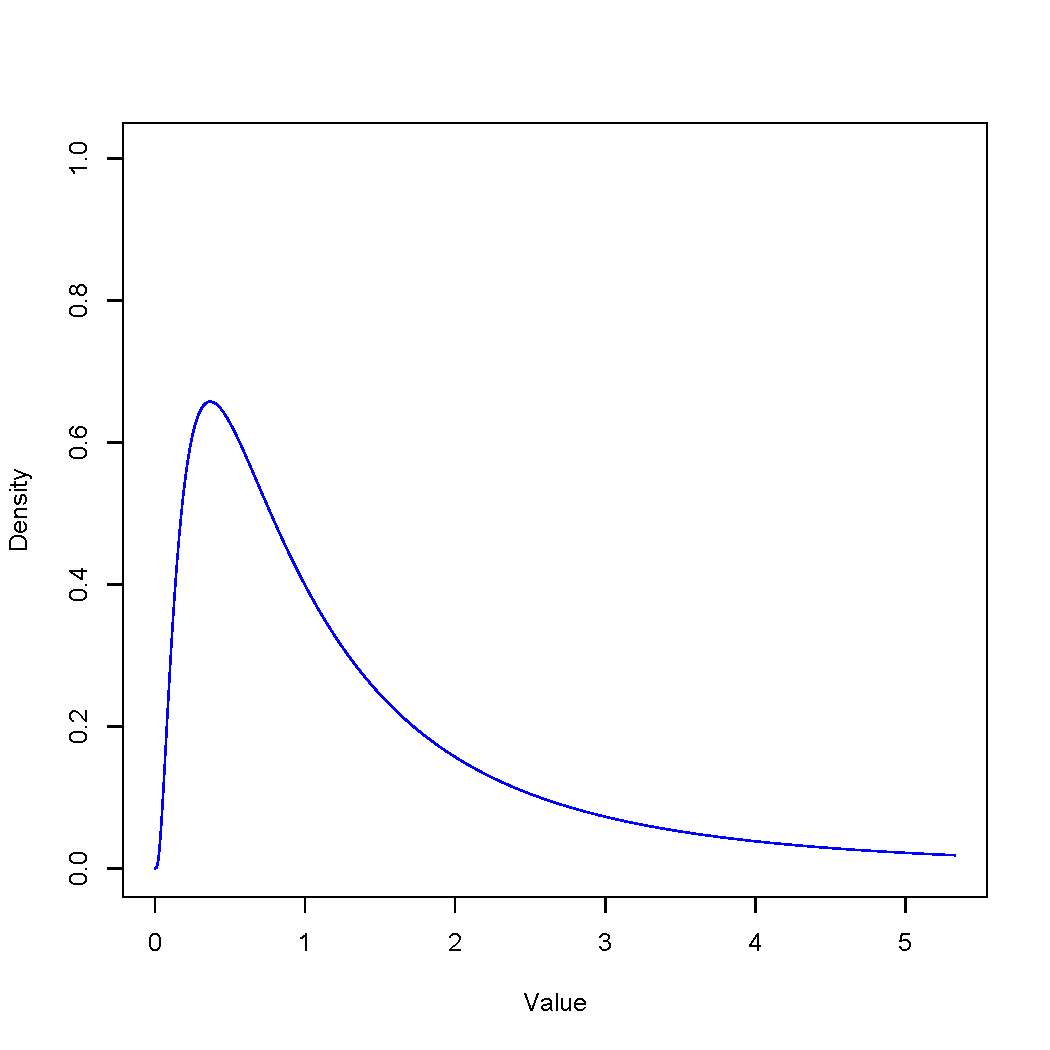
\includegraphics[width=1.0\textwidth]{Figure2}        
		\end{center}   
	 \end{column}    
	\begin{column}{5cm}        
	  
	\begin{itemize}
	\item Probability density that x is a certain value
	\item Based on a function - area below the curve must equal to 1
	\item Higher density indicates more likely the values given the distribution
	\end{itemize}
	\end{column}
	\end{columns}

\end{frame}

\begin{frame}{Probability  Distribution Functions (PDF)}
\begin{columns}    
	\begin{column}{4cm}        
		\begin{center}
		PDF Plot           
	 	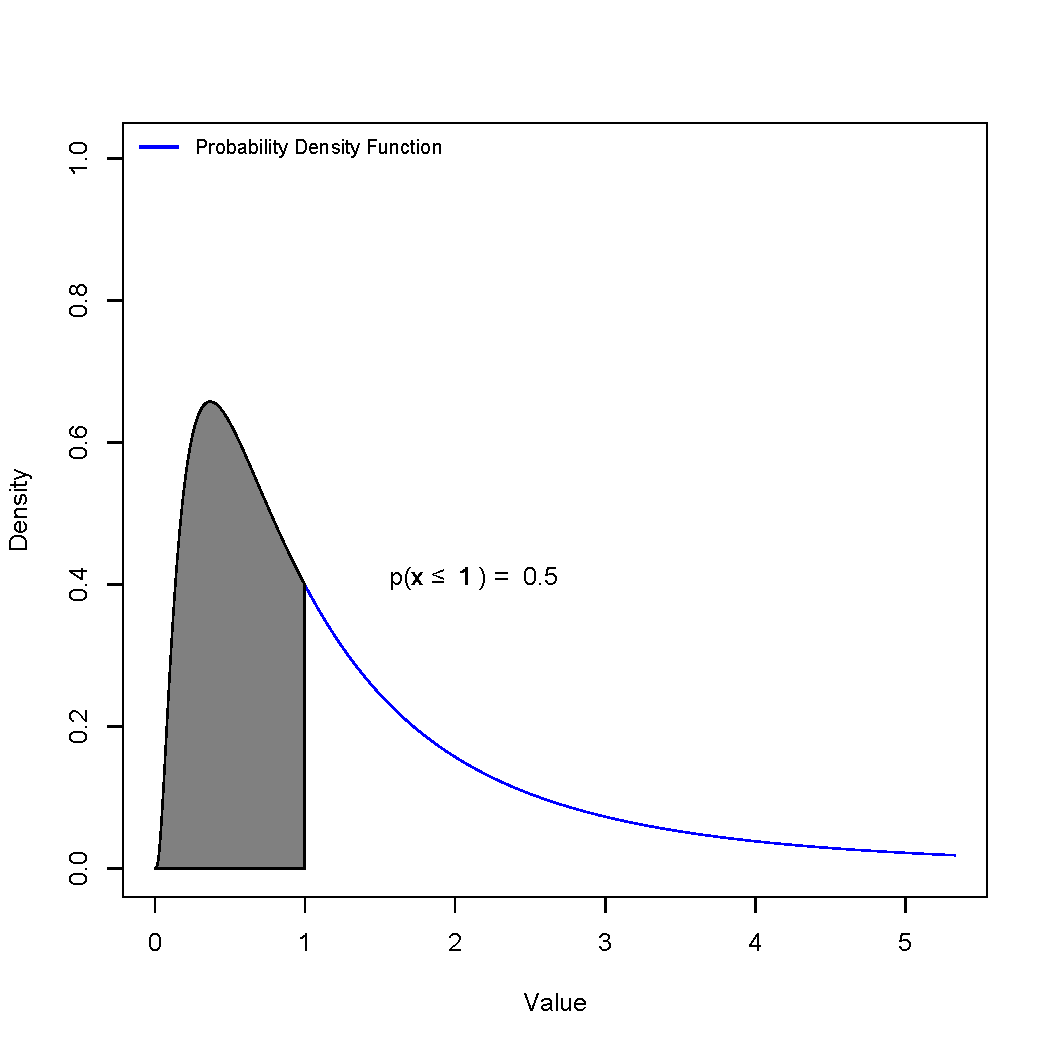
\includegraphics[width=1.0\textwidth]{Figure3}        
		\end{center}   
	 \end{column}    
	\begin{column}{5cm}        
	  
	\begin{itemize}
	\item PDF can be used to calculate that  x is within a range of values
	\item Equal to the area under the PDF curve below a given value
	\item Here we see probability $X \le 1$ is 0.5
	\end{itemize}
	\end{column}
	\end{columns}

\end{frame}


\begin{frame}{Cummulative  Distribution Functions (CDF)}
We can also plot the PDF another way – instead of the density on the y axis, we can plot the cumulative probability that  $X \le Value$. This is called the Cumulative Distribution Function (CDF).	
\begin{columns}    
	\begin{column}{4cm}        
		\begin{center}
		CDF Plot           
	 	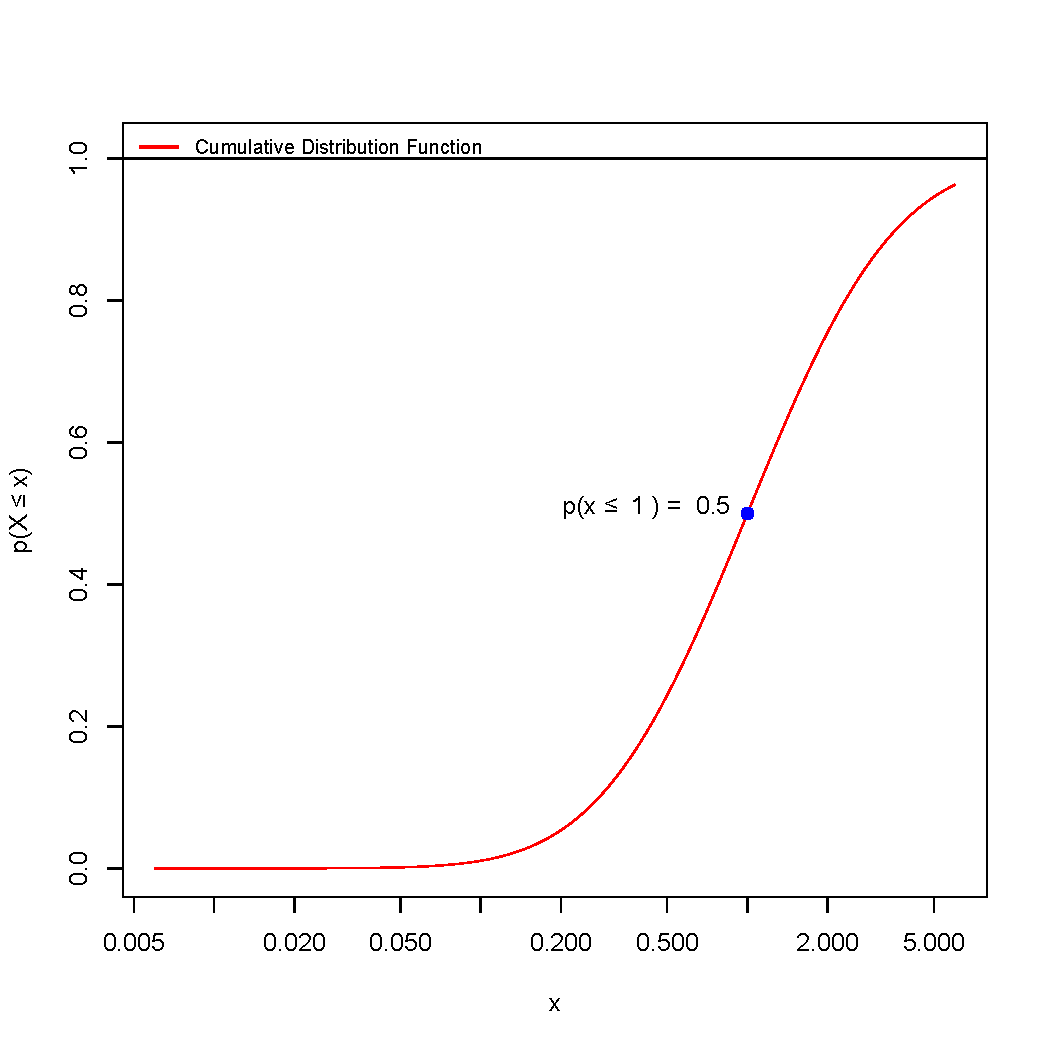
\includegraphics[width=1.0\textwidth]{Figure4}        
		\end{center}   
	 \end{column}    
	\begin{column}{5cm}        
	  
	\begin{itemize}
	\item CDF’s can be used to calculate mean
	\item Area of (Value x CDF(Value)) = mean
	\end{itemize}
	\end{column}
	\end{columns}

\end{frame}

\begin{frame}{ECDF and CDF}
ECDF approximates CDF	
\begin{columns}    
	\begin{column}{4cm}        
		\begin{center}
		ECDF and CDF Plot           
	 	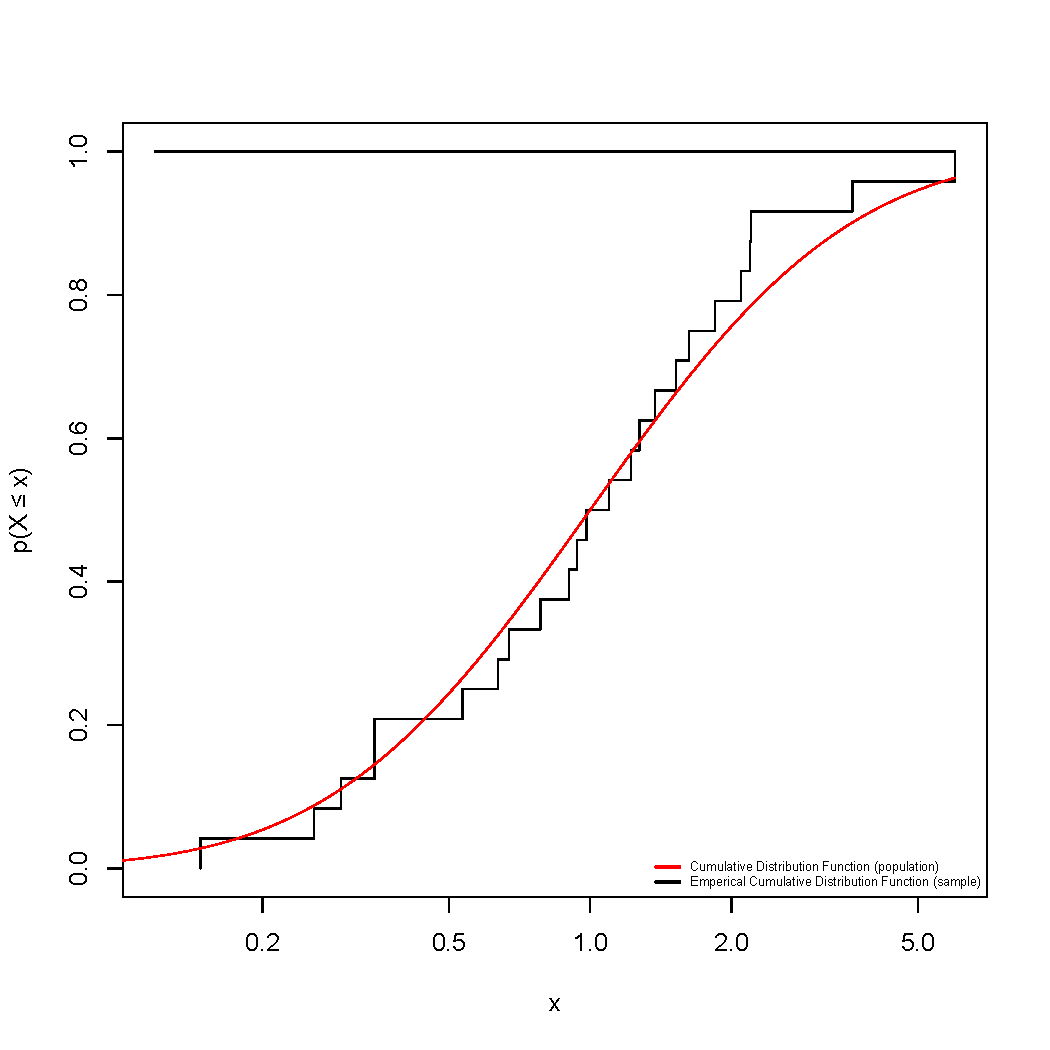
\includegraphics[width=1.0\textwidth]{Figure5}        
		\end{center}   
	 \end{column}    
	\begin{column}{5cm}        
	  
	\begin{itemize}
	\item BOTH can be used to calculate mean
	\item Area of (Value x CDF(Value)) = mean
	\item Area of (Value x ECDF(Value)) = mean
	\end{itemize}
	\end{column}
	\end{columns}

\end{frame}

\begin{frame}{Probability Plotting}

\begin{columns}    
	\begin{column}{4cm}        
		\begin{center}		           
	 	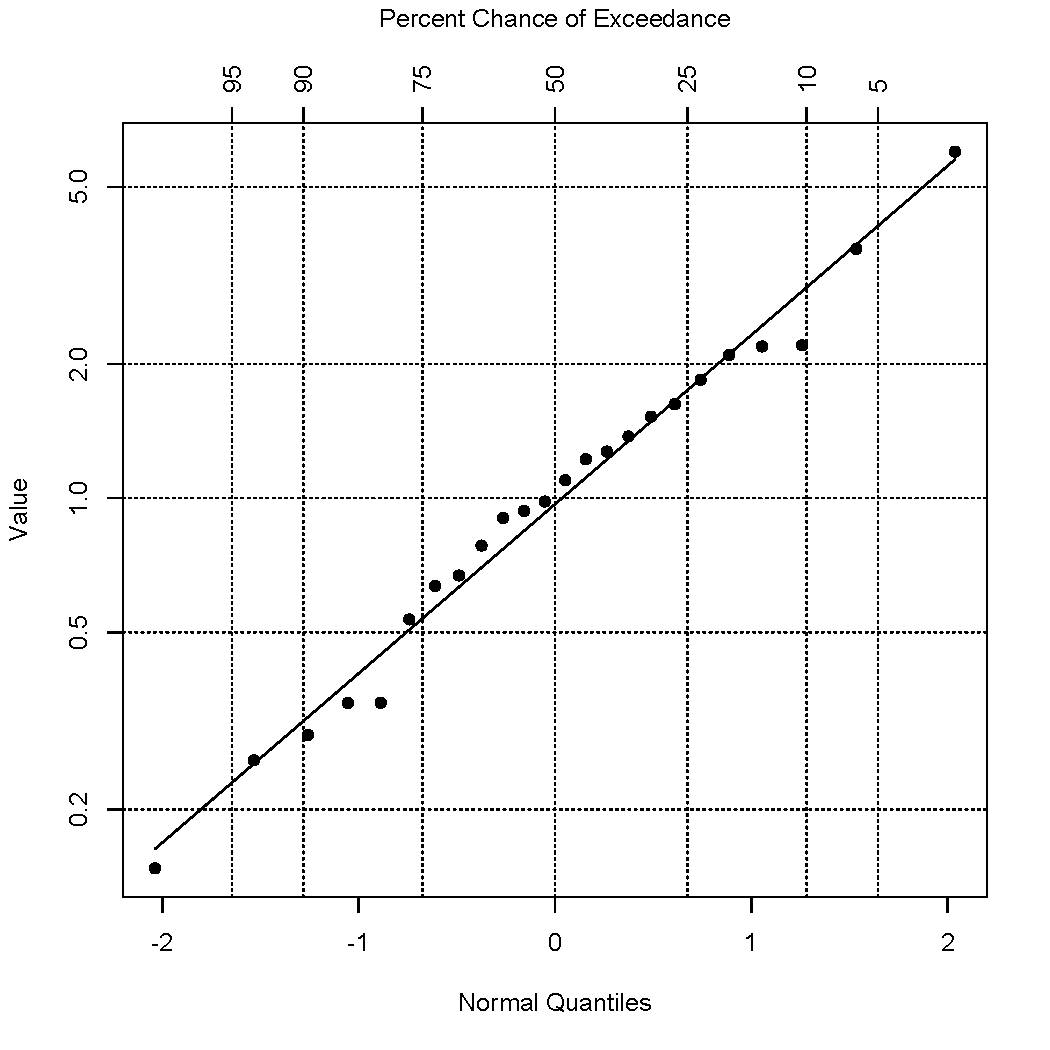
\includegraphics[width=1.0\textwidth]{Figure7}        
		\end{center}   
	 \end{column}    
	\begin{column}{5cm}        
	\begin{itemize}
	\item Compute plotting position (number of standard deviations)
	\item This is also a probability
	\item Plot values versus their probability on a scale of standard deviations
	\end{itemize}
	\end{column}
	\end{columns}

\end{frame}


\begin{frame}{Maximum Likelihood}
\begin{itemize}
\item With multiple observations, the likelihood of the parameters (e.g. mean and variance) is proportional to their probability densities given the parameters multiplied together
\begin{center}
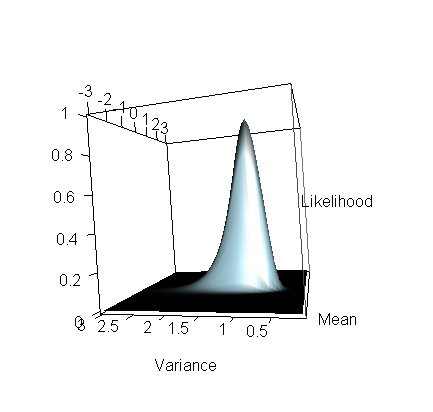
\includegraphics[height=6cm]{Figure8}
\end{center}
\end{itemize}
\end{frame}


\section{Censored Data Analysis}





\subsection{Kaplan-Meier}

\begin{frame}{Kaplan Meier - [KM] }

\end{frame}

\subsection{Robust Regression on Order Statistics}

\begin{frame}{Robust Regression on Order Statistics - [ROS] }

\end{frame}


\subsection{Maximum Likelihood Estimation}

\begin{frame}{Maximum Likelihood Estimation - [MLE] }

\end{frame}

\subsection{Multiple Imputation}

\begin{frame}{Multiple Imputation - [MI] }

\end{frame}



\section{Confidence Intervals}

\subsection{Parametric Confidence Intervals}

\begin{frame}{Choice of Parametric Distribution}

\end{frame}


\subsection{Bootstrapping}

\begin{frame}{The Bootstrap}

\end{frame}
 
\begin{frame}{Limitations of Bootstraps}

\end{frame}

\subsection{Chebychev Inequalities}

\begin{frame}{Chebychev Inequality}

\end{frame}


\end{document}


